\chapter{Experiments and Results}
\label{chapter:experiments}

This chapter summarizes the experiments carried out for our proposed model, the Softmax Mixture, and several pointer based models. We also discuss the results obtained when applying these models on the LAMBADA dataset.

All the experiments described in this chapter have been implemented using Tensorflow v1.4 \cite{tensorflow2015}. The code is publicly available at \url{https://github.com/moisestg/rare-lm}.

\section{Softmax Mixture Model}
\label{sec:smmExps}

\subsection{Experimental Setup}

The original LAMBADA dataset contains lowercased text. As will be described in the upcoming experiments section, part of our preprocessing requires PoS tagging the text. Although there are caseless PoS taggers available, in order to maximize the accuracy of this step we opted to use the capitalized version of the dataset\footnote{Available at \url{http://clic.cimec.unitn.it/lambada/train-novels-capitalized.txt.gz}}.

Additionally, we delimited each novel in the corpus with a special a tag and used that to randomize the order in which the novels are fed to the model for each epoch.

Furthermore, following the recommendations from \cite{merity2016pointer} we modified our base code resulting in a much faster implementation: During the training phase it is only necessary to compute the softmax probability of the target word (rather than the whole vocabulary) in order to compute the cross-entropy loss, as the observed distribution is a one-hot encoding of the correct output.

Finally, \autoref{trainSmm} summarizes the specific training configuration used in the following set of experiments:

\begin{table}[]
	\centering
\begin{tabular}{|c|c|}
	\hline
	\textbf{Training data}                                                     & 1/3 of all the training novels                                                              \\ \hline
	\textbf{Development data}                                                  & \begin{tabular}[c]{@{}c@{}}100K contiguous sentences\\  from the remaining 2/3\end{tabular} \\ \hline
	\textbf{Vocabulary size}                                                   & 44636                                                                                       \\ \hline
	\textbf{Word embeddings}                                                   & \begin{tabular}[c]{@{}c@{}}150-d word2vec (pretrained\\ on the training data)\end{tabular}  \\ \hline
	\textbf{Optimizer}                                                         & \begin{tabular}[c]{@{}c@{}}ADAM with learning \\ rate of 0.001 \end{tabular}             \\ \hline
	\textbf{TBPPT}                                                             & $k_1=1$ and $k_2=20$                                                                        \\ \hline
	\textbf{Batch size}                                                        & 64                                                                                          \\ \hline
	\textbf{\begin{tabular}[c]{@{}c@{}}Maximum global \\ L2 norm\end{tabular}} & 8                                                                                           \\ \hline
	\textbf{Training epochs}                                                     & 10 \\ \hline
\end{tabular}
	\caption{Training configuration for \autoref{sec:smmExps}.}
	\label{trainSmm}
\end{table}

\subsection{Regularization Experiments}
\label{sec:regExps}

As described in \autoref{sec:mixtureModel}, the Softmax Mixture model has the ability to encode two differentiated output distributions that are dynamically blended by the switching network. In order to train the switching component in a supervised fashion, we need to tag each word in the training set with its corresponding source. 

Motivated by our initial analysis of LAMBADA, we decided to tag peoples' names as they are a very specific subset of rare words that a vanilla softmax output layer fails to handle. By using a predefined list\footnote{Available at \url{https://deron.meranda.us/data/}.}, we also made sure to reduce the amount of false positives (at the expense of missing some rare or fictitious names).

In our first batch of experiments we started exploring the space of hyperparameters by finding an optimal value for $\lambda$, the weight of the loss term in charge of the training supervision of the switching component. \autoref{fig:lambdaPerplexity} shows the evolution of the development perplexity during training for the explored range of values. We can see that values of $\lambda$ up to 100 produce a similar behavior on the overall perplexity of the model. Higher values start to noticeably hinder the learning process as the sigmoid loss of the switching component starts to overcome the cross-entropy loss.

\begin{figure}[H]
	\centering
	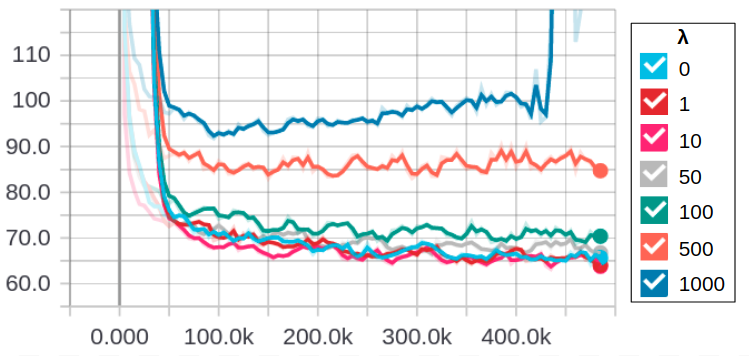
\includegraphics[scale=0.4]{lambdaPerplexity}
	\captionof{figure}{Development perplexity traces for different values of lambda.}
	\label{fig:lambdaPerplexity}
\end{figure}

As already discussed in \autoref{sec:problemRare}, the behavior of rare words is masked when studying the overall performance of a model. A set of preliminary experiments where we studied the performance of names in isolation revealed the existence of two differentiated regimes. In particular, \autoref{fig:perplexityRare} shows the training traces for baseline language model consisting of a single-layered LSTM with 512 hidden units (following the recommendations from \cite{paperno2016lambada}), where a clear overfitting trend is observed for names.

These discoveries led us to run a collection of experiments summarized in \autoref{smmExps}, where we studied the behavior of the baseline and one specific configuration of our model ($\lambda=100$) when applying different regularization techniques on them: 

\begin{table}[H]
	\centering
	\makebox[\textwidth][c]{\begin{tabular}{cc|c|c|c|c|}
		\cline{3-6}
		\multicolumn{1}{l}{}                                                    & \multicolumn{1}{l|}{}   & \multicolumn{2}{c|}{\textbf{All words}} & \multicolumn{2}{c|}{\textbf{Names}} \\ \cline{3-6} 
		&                         & \textbf{Train}       & \textbf{Dev}        & \textbf{Train}        & \textbf{Dev}         \\ \hline
		\multicolumn{1}{|c|}{\multirow{2}{*}{\textbf{No regularization}}}                            & \textbf{\textbf{Baseline}}                & 42.5        & 61.5       & 1K         & 130K        \\ \cline{2-6} 
		\multicolumn{1}{|c|}{}                                                  & \textbf{Mixture ($\boldsymbol{\lambda}\mathbf{=100}$)} & 55          & 69         & 4K         & 120K        \\ \hline
		\multicolumn{1}{|c|}{\multirow{2}{*}{\textbf{Input dropout}}}                    & \textbf{Baseline}                & 52.5        & 63         & 2K         & 140K        \\ \cline{2-6} 
		\multicolumn{1}{|c|}{}                                                  & \textbf{Mixture ($\boldsymbol{\lambda}\mathbf{=100}$)} & 65          & 72         & 8K         & 120K        \\ \hline
		\multicolumn{1}{|c|}{\multirow{2}{*}{\textbf{Hidden state dropout}}}                    & \textbf{Baseline}                & 48          & 62.5       & 1K         & 120K        \\ \cline{2-6} 
		\multicolumn{1}{|c|}{}                                                  & \textbf{Mixture ($\boldsymbol{\lambda}\mathbf{=100}$)} & 62.5        & 73         & 6K         & 120K        \\ \hline
		\multicolumn{1}{|c|}{\multirow{2}{*}{\textbf{Output dropout}}}                   & \textbf{Baseline}                & 62.5        & 65         & 5K         & 150K        \\ \cline{2-6} 
		\multicolumn{1}{|c|}{}                                                  & \textbf{Mixture ($\boldsymbol{\lambda}\mathbf{=100}$)} & 80          & 73         & 20K          & 80K         \\ \hline
		\multicolumn{1}{|c|}{\multirow{2}{*}{\textbf{L2 regularization ($\text{weight}\mathbf{=0.01}$)}}} & \textbf{Baseline}                & 100         & 125        & 10K          & 400K        \\ \cline{2-6} 
		\multicolumn{1}{|c|}{}                                                  & \textbf{Mixture ($\boldsymbol{\lambda}\mathbf{=100}$)} & 107.5       & 119        & 8K         & 120K        \\ \hline
	\end{tabular}}
	\caption{Perplexity for different regularization techniques.}
	\label{smmExps}
\end{table}

Specifically we tested variational dropout applied separately on the input, outputs and hidden state units\footnote{Tensorflow's \texttt{DropoutWrapper} implementation of variational dropout for the hidden state is only functional from v1.4 onwards.} using $p=0.5$. We also tried including an L2 regularization term applied on the weights of the softmax layers. The results indicate that none of the approaches is able to improve on the unregularized baseline in terms of overall perplexity (61.5 on the development set). However if we focus our attention on names, we can see that our model in combination with output dropout reduces the perplexity of the baseline in 40\%.

\autoref{fig:outDropPerplexities} shows some additional experiments that focus on the effect of output dropout on our model, featuring different combinations of $\lambda$ and $p$ and splitting the results depending on whether a word was tagged as a name. In general we observe that for words that are not names, the models benefit from lighter (higher keep probability) dropout while for names, all configurations exhibit a very similar behavior.

\begin{figure}[H]
	\centering
	\makebox[\textwidth][c]{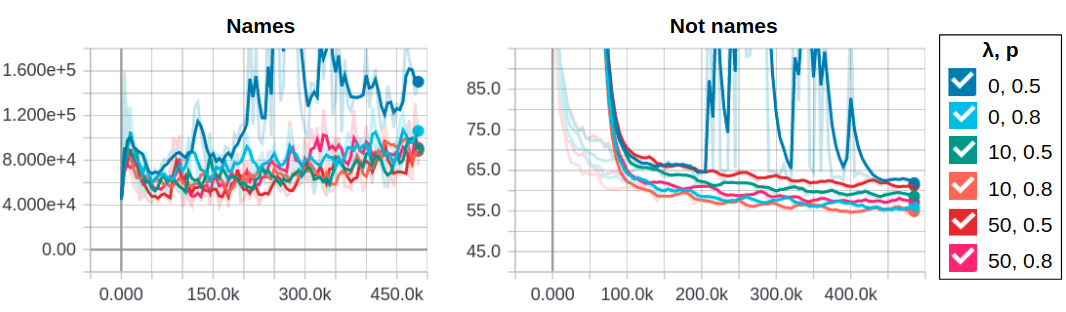
\includegraphics[scale=0.425]{outDropPerplexities}}
	\captionof{figure}{Development perplexity traces for different combinations of lambda and output keep probability.}
	\label{fig:outDropPerplexities}
\end{figure}

\begin{table}[H]
	\centering
	\begin{tabular}{cc|c|c|}
		\cline{3-4}
		&                                                                                                               & \textbf{Names} & \textbf{Not names} \\ \hline
		\multicolumn{1}{|c|}{\multirow{3}{*}{$\boldsymbol{\lambda}\mathbf{=10}$}} & $\mathbf{p=0.5}$                                                                                              & 62K            & 59                 \\ \cline{2-4} 
		\multicolumn{1}{|c|}{}                                                    & $\mathbf{p=0.8}$                                                                                              & 65K            & 54                 \\ \cline{2-4} 
		\multicolumn{1}{|c|}{}                                                    & 
		$\mathbf{p_1}=0.8,\mathbf{p_2}=0.625$   & 61K            & 54                 \\ \hline
		\multicolumn{1}{|c|}{\multirow{3}{*}{$\boldsymbol{\lambda}\mathbf{=50}$}} & $\mathbf{p=0.5}$                                                                                              & 60K            & 61                 \\ \cline{2-4} 
		\multicolumn{1}{|c|}{}                                                    & $\mathbf{p=0.8}$                                                                                              & 61K            & 57                 \\ \cline{2-4} 
		\multicolumn{1}{|c|}{}                                                    & 
		$\mathbf{p_1}=0.8,\mathbf{p_2}=0.625$ & 60K            & 57                 \\ \hline
	\end{tabular}
	\caption{Development perplexity comparison between regular and splitted dropout.}
	\label{splittedDropPerplexities}
\end{table}

As already discussed, all previous experiments have shown differentiated dynamics for names and not names. Inspired by this, we decided to try a modified version of variational dropout, called \textit{splitted dropout}, to be used in combination with our softmax mixture model. The basic idea is being able to apply different regularization strengths for the output distributions of names and not names. 

The procedure is summarized in \autoref{eq:splittedDropout}: We first sample two dropout masks $\mathbf{m_1},\mathbf{m_2}$ (with keep probabilities $p_1$ and $p_2$, respectively) of the same size of the hidden states. The mask that will be use for not names is equal to $\mathbf{m_1}$. To obtain the mask for names, we calculate the element-wise product of $\mathbf{m_1}$ and $\mathbf{m_2}$. With this approach we ensure that the zeros from the not names' mask are preserved, maximizing the overlap of the dropped units in both masks. We then apply both masks to the sequence of hidden states. The sequence with lighter dropout (keep probability of $p_1$) is then fed to the softmax layer encoding the distribution of not name words while the sequence with heavier dropout (keep probability of $p_1p_2$) is fed to the layer names' softmax layer.

\begin{equation} \label{eq:splittedDropout}
\begin{gathered}
	\mathbf{m_1} \sim \text{Dropout}(p_1) \\
	\mathbf{m_2} \sim \text{Dropout}(p_2) \\
	\mathbf{m_{\text{not names}}} = \mathbf{m_1}, \; \mathbf{m_{\text{names}}} = \mathbf{m_1} \odot \mathbf{m_2}) \\
	p(m_{\text{names}} \neq 0) = p(m_1 \neq 0 \wedge m_2 \neq 0) = p_1 p_2
\end{gathered}
\end{equation}

where $\mathbf{m_1},\mathbf{m_2} \in \mathbb{R}^h$.

\autoref{splittedDropPerplexities} compares the results obtained with regular variational dropout and splitted dropout. Selecting $p_1=0.8$ and $p_2=0.625$ is equivalent to applying dropouts with keep probabilities of 0.8 and 0.5 for not names and names, respectively. We can observe that the proposed variant allows for stronger dropout of the names distribution without impacting the overall performance.

\subsection{Switch Component Experiments}

We have just seen that none of the tested configurations for the softmax mixture managed to improve on the baseline in terms of overall perplexity. In this section, we detail a series of experiments that were carried out to determine the performance of the switching component and check if this may be cause for the results obtained so far.

As a first step, we decided to study the performance of the classifier in isolation. To do that we used a confusion matrix, one of the standard evaluation tools for classifier evaluation. \autoref{confMatrix} shows the results obtained by the classifier on the development set:

\begin{table}[H]
	\centering
	\begin{tabular}{cc|c|c|}
		\cline{3-4}
		&                   & \multicolumn{2}{c|}{\textbf{Prediction}} \\ \cline{3-4} 
		&                   & \textbf{Name}     & \textbf{Not name}    \\ \hline
		\multicolumn{1}{|c|}{\multirow{2}{*}{\textbf{\begin{tabular}[c]{@{}c@{}}Ground\\ Truth\end{tabular}}}} & \textbf{Name}     & 20859             & 20292                \\ \cline{2-4} 
		\multicolumn{1}{|c|}{}                                                                                 & \textbf{Not name} & 123220            & 1874029              \\ \hline
	\end{tabular}
	\caption{Confusion matrix for the name classifier (threshold=0.5).}
	\label{confMatrix}
\end{table}

First of all, we can observe the strong imbalance present in our dataset, with names constituting only 2\% of all words. This prevented us from using biased metrics when applied to highly-skewed data such as accuracy (93\% in this example). Instead we defined names to be our positive class and used precision, recall and $F_1$ score as our metrics. 

\begin{equation} \label{eq:classResults}
\begin{gathered}
	P = \frac{TP}{TP+FP} = \frac{20859}{20859+123220} = 0.14 \\
	R = \frac{TP}{TP+FN} = \frac{20859}{20859+20292} = 0.51 \\
	F_1 = 2 \frac{P\cdot R}{P+R} = 0.23
\end{gathered}
\end{equation}

The results from \autoref{eq:classResults} clearly show that the performance of the classifier for names is very poor. In an attempt to mitigate this imbalance problem, several techniques were applied. Namely, undersampling of the majority class (by reducing the ratio of not names/names from its initial value of 50 to 1) and introducing a class weight for names in the loss function so errors made on names are more costly. However none of our efforts rendered any noticeable performance gains.

Qualitative inspection of the results seemed to suggest that independently from the imbalance in the data, predicting if an upcoming word is a name given the previous ones is inherently a hard problem. The classifier manages to predict names confidently only when they are strongly cued in the previous context. Examples of this would be the end of a character's dialogue line followed by the word ``said'' (which are quite common in literary texts such as LAMBADA) or after personal titles such as ``Mr.''. However, more general situations are much harder as common nouns and personal pronouns can be usually used in the same locations as names.

Based on our previous findings, we hypothesized that the switching component was the limiting factor for our softmax mixture model. In order to validate this, we ran an additional experiment where the output of the switching component $p(z_t=1|\mathbf{h}(t))$ was substituted with the ground truth: 

\begin{table}[H]
	\centering
	\begin{tabular}{c|c|c|}
		\cline{2-3}
		& \textbf{Names}        & \textbf{All words}  \\ \hline
		\multicolumn{1}{|c|}{\multirow{3}{*}{\textbf{Ground truth}}}                                                                & \multirow{3}{*}{5K} & \multirow{3}{*}{57} \\
		\multicolumn{1}{|c|}{}                                                                                                      &                       &                     \\
		\multicolumn{1}{|c|}{}                                                                                                      &                       &                     \\ \hline
		\multicolumn{1}{|c|}{\multirow{3}{*}{\textbf{\begin{tabular}[c]{@{}c@{}}Ground truth and\\ splitted dropout\\$\mathbf{p_1}=0.8,\mathbf{p_2}=0.625$\end{tabular}}}} & \multirow{3}{*}{4K} & \multirow{3}{*}{55} \\
		\multicolumn{1}{|c|}{}                                                                                                      &                       &                     \\
		\multicolumn{1}{|c|}{}                                                                                                      &                       &                     \\ \hline
	\end{tabular}
	\caption{SMM perplexity with ground truth switching.}
	\label{groundTruthPerplexities}
\end{table}

The results in \autoref{groundTruthPerplexities} show that with this configuration, our model manages to improve on the baseline in overall perplexity (4.5 perplexity points lower down to 57), mainly due to the great reduction of perplexity for names. Additionally, applying the splitted dropout technique described earlier provides further performance gains.

As we detailed in \autoref{sec:mixtureModel}, our model aims to learn two differentiated output distributions for names and not names. \autoref{top10forNames} shows the top ten predictions made for several words tagged as names\footnote{``England'' and ``English'' are very popular english last names}. These examples show that our model successfully learns better suited output distributions for names, shifting the probability mass towards names. 

\begin{table}[H]
	\centering
	\begin{tabular}{|c|c|c|c|}
		\hline
		Lily & Rachel & England & English \\ \hline
		\makecell{Dean\\Xavier\\David\\Lily\\Noah\\Al\\Alex\\Hunter\\Eric\\Derek} & \makecell{Caroline\\Hunter\\Elizabeth\\Emma\\David\\Julia\\Trevor\\Zoe\\Dan\\Kim} & \makecell{London\\America\\England\\Santa\\Paris\\France\\Little\\North\\Paul\\English} & \makecell{English\\French\\Christian\\Irish\\German\\Roman\\Marine\\Fae\\Dean\\Sunday} \\ \hline
	\end{tabular}
	\caption{Top 10 predictions for words tagged as names.}
	\label{top10forNames}
\end{table}

Additionally, we also studied how ``different'' were the average output distributions for names and not names. For this we used the Jensen-Shannon divergence, a metric for measuring the similarity between probability distributions. While experiments from \autoref{sec:regExps} were producing average divergence values of 0.21, experiments from \autoref{groundTruthPerplexities} reported average divergences of 0.69 (very close to the its upper bound value for our setting, $\ln(2)$). These results seem to confirm that our model is successfully learning two differentiated output distributions.

Finally, we wanted to test the behavior of our model when rather than making a distinction between names and not names (a hard task based on our previous results), we differentiate between nouns and not nouns (we considered as nouns words marked as common or proper nouns by the default \texttt{Stanford PoS tagger}\footnote{\texttt{NN,NNS} and \texttt{NNP,NNPS}, respectively}). Initial results seem to indicate that while the switch component is able to classify words more confidently, the divergence drops back to 0.21 and overall perplexity is in the same range as name models. A possible explanation for this could be modeling the output distribution of common and proper nouns together might be dominated by common nouns as they are much more frequent. However, further experiments would be required to check this.

\section{Pointer Based Models}
\label{sec:pointerExps}

\subsection{Experimental Setup}

The experiments described in this section are evaluated on the LAMBADA task so we follow the training methodology described in \cite{paperno2016lambada}. Namely, we train on the full lowercased training set and use a vocabulary size of 93215. Additionally, we incremented the dimension of our word embeddings to 200. For training the pointer sentinel mixture model we used TBPTT with $k_2=100$ as in \cite{merity2016pointer}.

An important detail when training the PSMM is the initialization of the sentinel vector $\mathbf{s}$. If initialized with too large values, the last element of $\mathbf{z}$, corresponding to the logit of the gate, will be much bigger than the rest and applying the softmax will lead to $g_t=1$. If this is the case, the loss will be equal to the regular cross-entropy loss (as shown in \autoref{eq:psmmGrad}) and the pointer component won't be trained.

\begin{equation} \label{eq:psmmGrad}
\begin{gathered}
\mathcal{L}(\theta) = -\log(g_t \, p_{\text{vocab}}(w=y(t)|\mathbf{h}(1\ldots t)) + \sum_{k \in I(y(t), \; x(t))}\mathbf{a}(t)_k) \\
-\log(g_t + \sum_{i \in I(y(t), \; x(t))}\mathbf{a}(t)_i) \stackrel{g_t=1}{=} -\log(p_{\text{vocab}}(w=y(t)|\mathbf{h}(1\ldots t))
\end{gathered}
\end{equation}

\subsection{Experiments}

To finish this chapter, we describe the experiments carried out with the PSMM and describe its performance when applied to the LAMBADA task. \autoref{psmmExps} summarizes the obtained results for the baseline described in \autoref{sec:regExps}, the neural continuous cache model introduced in \autoref{sec:continuousCache} and the pointer sentinel mixture model also introduced in \autoref{sec:pointerMixture}.

\begin{table}[H]
	\centering
	\begin{tabular}{c|c|c|}
		\cline{2-3}
		\multicolumn{1}{l|}{}                            & \textbf{Control} & \textbf{LAMBADA} \\ \hline
		\multicolumn{1}{|c|}{\textbf{LSTM-512} \cite{paperno2016lambada}}          & 149              & 5357             \\ \hline
		\multicolumn{1}{|c|}{\textbf{Continuous Cache} \cite{grave2016improving}}               & 129              & 138              \\ \hline
		\multicolumn{1}{|c|}{\textbf{PSMM (length=100)}} & 114              & 154              \\ \hline
		\multicolumn{1}{|c|}{\textbf{PSMM (length=200)}} & 116              & 172              \\ \hline
	\end{tabular}
	\caption{Perplexity on LAMBADA.}
	\label{psmmExps}
\end{table}

We can observe that the PSMM with a pointer window of 100 words improves upon the continuous cache on the control set and gets worse but comparable results on LAMBADA. It is important to note that the parameters of the continuous cache model (the interpolation weight and the sharpness parameter for the cache distribution) were manually tuned to maximize the performance on each set. On the contrary, the PSMM learnt all its parameters automatically.

This makes the PSMM specially appealing as it does not make any assumptions on the text that is going to be evaluated on. Furthermore, by calculating the mixture gate $g_t$ for each word it allows to inspect the dynamics of the model in a more intuitive way. 

For example, \autoref{fig:gateEx2} illustrates a LAMBADA passage where the model is very confident that the next word is contained in the window (low $g_t$, probably due to the word ``miss'') and successfully shifts the probability mass to the previous occurrence of the target word.

\begin{figure}[H]
	\centering
	\makebox[\textwidth][c]{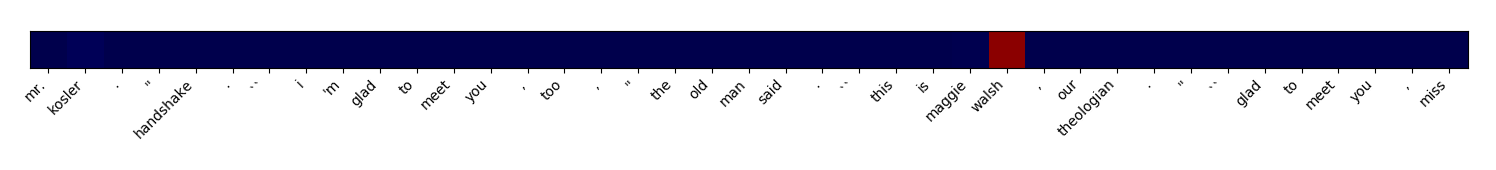
\includegraphics[scale=0.305]{gatesEx2}}
	\captionof{figure}{Predicting ``walsh'' ($g_t=0.07$).}
	\label{fig:gateEx2}
\end{figure}

In \autoref{fig:gateEx1} we see that although the target word is a common name, the model successfully identifies the repeated pattern ``out of the fort'' and assigns the highest probability to the two previous occurrences.

\begin{figure}[H]
	\centering
	\makebox[\textwidth][c]{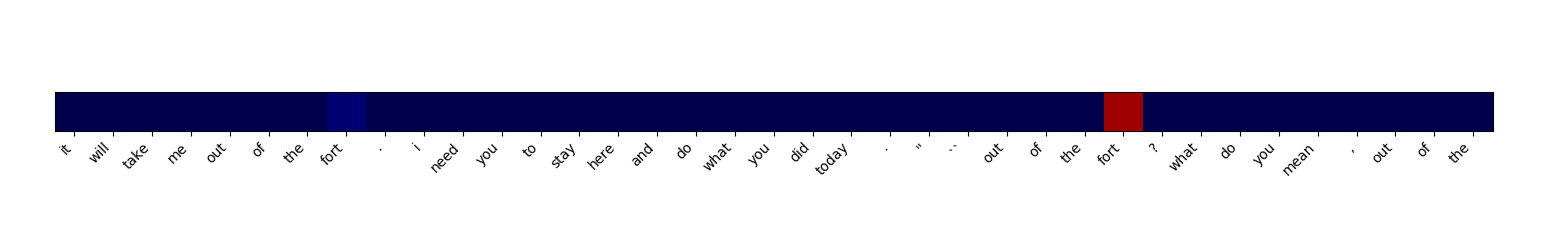
\includegraphics[scale=0.3]{gateEx1}}
	\captionof{figure}{Predicting ``fort'' ($g_t=0.28$).}
	\label{fig:gateEx1}
\end{figure}

Finally, \autoref{fig:gateEx3} shows that the model is also able to identify situations where the pointer is not likely to help.

\begin{figure}[H]
	\centering
	\makebox[\textwidth][c]{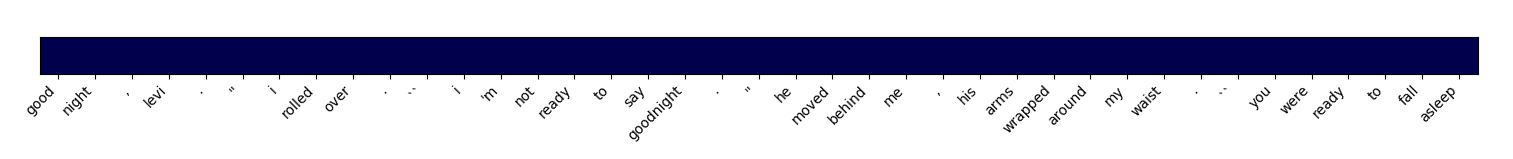
\includegraphics[scale=0.3]{gateEx3}}
	\captionof{figure}{Predicting ``earlier'' ($g_t=0.99$).}
	\label{fig:gateEx3}
\end{figure}